\subsubsection{Als Entwickler registrieren}

\begin{figure}[H]
    \begin{center}
      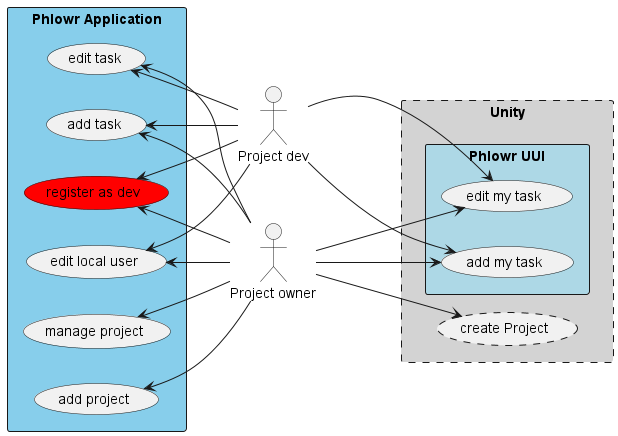
\includegraphics[width=0.3\linewidth]{../content/diagrams/usecase/overview/overviewUseCaseRegisterAsDevSelected.png}
      \caption{Use Case Diagaramm <register as dev> }
    \end{center}
  \end{figure}

   \begin{table}[H]
    \centering
    \settowidth\tymin{executeIncomingCommand()}
    \setlength\extrarowheight{2pt}
    \begin{tabulary}{1.0\textwidth}{|m{4cm}|m{9cm}|}
      \hline
      \textbf{Use Case} &
      \textbf{REGISTER AS DEV}\\
      \hline
      \textbf{Beschreibung} &
      Ein User registriert sich bei einem Projekt.
      Dies ist nötig, damit der User zur Planung im Projekt zu Verfügung steht.\\ 
      \hline
      \textbf{Includes} &
      \begin{itemize}
       \item keine
        \end{itemize}\\ 
        \hline 
      \textbf{Akteure} &
      Entwickler\\ 
      \hline
      \textbf{Auslöser} &
      \begin{itemize}
        \item ein Entwickler möchte an einem Projekt mitarbeiten
         \end{itemize}\\  
      \hline
      \textbf{Vorbedingungen} &
      \begin{itemize}
        \item es ist ein freier Slot im Projekt verfügbar
        \item der Entwickler ist im Projekt noch nicht registriert
        \item das Projekt ist auf dem aktuellsten Stand
      \end{itemize}\\  
      \hline
      \textbf{Abschlussbedingunen} &
      Der User ist im Projekt zur plan verfügbar 
      Der User kann für sich selbst Tasks im Projekt erstellen\\
      \hline
      \textbf{Ablauf} &
      \begin{enumerate}
        \item Applikation öffnen
        \item Projekt öffnen
        \item <Als Entwickler Registrieren> klicken
        \item Speichern
        \item falls nötig Projekt synchronisieren
        \end{enumerate}\\ 
      \hline
      \textbf{Zu Beachten / Notizen} &
      \begin{itemize}
        \item das Projekt muss auf dem neusten Stand sein -> es könnten Merge-Konflikte auftreten
        \end{itemize}\\ 
      \hline
    \end{tabulary}
    \caption{Use Case: register as dev}
  \end{table}
